\documentclass{article}
\usepackage{preamble}
\title{Constraint Solver Implementation}
\author{140011146}

\makeatletter
\let\thetitle\@title
\let\theauthor\@author
\let\thedate\@date
\makeatother

\begin{document}


\maketitlepage{CS4402 Constraint Programming}{Ian Miguel}




\section{Introduction}
In this practical, a forward checking constraint solver with 2-way branching is implemented. The implementation provides an interface to allow different heuristics for variable and value selection. To test the solver works as intended, problem instances of the N-queens, langfords and sudoku problems were generated and solutions created. Further, tests were written to ensure the right number of solutions were found for problem instances, for example exactly 724 solutions to the 10-queens problem. Finally, the performance of the solver and different heuristics are tested empirically using various metrics to explore and understand their differences. 

\section{Design and Implementation}
Many of the algorithms presented in this section were taken and adapted from the lecture slides to provide a complete method of what was done and any changes made during the implementation when compared to the original algorithm. 
\subsection{2 way forward checking}
The 2 way forward checking algorithm was implemented from the following algorithm:
\begin{algorithm}[H]
\begin{algorithmic}[1]
\Procedure{ForwardChecking}{\textit{varList}}
\If{completeAssignment()}
	\State addSolution()
\ElsIf{empty(\textit{varList})}
	\Return
\Else
	\State \textit{var} \gets selectVar(\textit{varList})
	\State \textit{val} \gets selectVal(domain(\textit{var}))
	\State branchFCLeft(\textit{varList}, \textit{var}, \textit{val})
	\State branchFCRight(\textit{varList}, \textit{var}, \textit{val})
\EndIf
\EndProcedure
\end{algorithmic}
\caption{2-way forward checking algorithm, adapted from lecture slides by Ian Miguel.}
\end{algorithm}
The small change made to the algorithm was to not exit when the first solution was found, but to add that solution to a list and continue to find more solutions. This was done to allow all solutions to be found as a means of testing the solver is working properly.
% A boolean variable was also added to stop the solver on the first solution found if needed. This was important to be able to experiment on the differences between finding one solution and finding all solutions, especially for larger constraint problems. 
To check for \texttt{completeAssignment()}, all variables in the problem instance contained a boolean to indicate that they have been assigned. \texttt{completeAssignment()} is true if all the variables are assigned. The variables can further be unassigned later by changing the assignment boolean in the corresponding variable.  
\n
The two methods \texttt{selectVar()} and \texttt{selectVal()} are implemented using heuristics which are explained below in section \ref{sec:heuristics}. Each heuristic implements its own variable and value selection functions which the solver uses, allowing the solver to be generic and extensible over any heuristic. Further, this means the heuristics do not have to worry about any other part of the solver, as the list of variables and domain of values are updated and kept track of in the solver to be passed to the heuristics. 
\n
Next, we look into detail on the algorithms for left and right branching.
\begin{algorithm}[H]
\begin{algorithmic}[1]
\Procedure{branchFCLeft}{\textit{varList}, \textit{var}, \textit{val}}
\State assign(\textit{var}, \textit{val})
\If{reviseFutureArcs(\textit{varList}, \textit{var})}
	\State ForwardChecking(\textit{varList} - \textit{var})
\EndIf
\State undoPruning()
\State unassign(\textit{var}, \textit{val})
\EndProcedure
\end{algorithmic}
\caption{Branching left during forward checking.}
\end{algorithm}
When we branch left, the selected value is assigned to the selected variable and future arcs revised. The idea is to ensure that for any particular value assignment, the arcs are revised to ensure local arc consistency. If the arc is still consistent, then we explore further down the tree by recursively forward checking with the reduced list of variables.
\n
When the functions eventually return or if the arc is inconsistent, the current value assignment does not lead to a solution, so any pruning done during arc revision must be undone for backtracking as the value assignment has not worked out. This is done with the \texttt{UndoTracker} class which keeps a map of each variable and the list of pruned values that need to be undone. Next, the solver contains a map of each variable to an \texttt{UndoTracker}. Whenever arcs are revised, the tracker for the variable chosen for revision is updated with the list of other future variables and their pruned values. This works to prune only values from each step of the recursion, because every time the algorithm goes down the left branch, a new variable is selected to be assigned and its arc revised. So when coming back up the tree, each depth corresponds directly to the selected variable, which acts as the key to an \texttt{UndoTracker}. 

\begin{algorithm}[H]
\begin{algorithmic}[1]
\Procedure{branchFCRight}{\textit{varList}, \textit{var}, \textit{val}}
\State deleteVal(\textit{var}, \textit{val})
\If{\neg\ empty(domain(\textit{var}))}
	\If{reviseFutureArcs(\textit{varList}, \textit{var})}
		\State ForwardChecking(\textit{varList})
	\EndIf
	\State undoPruning()
\EndIf
\State restoreVal(\textit{var}, \textit{val})
\EndProcedure
\end{algorithmic}
\caption{Branching right during forward checking.}
\end{algorithm}
As this is a 2-way branching scheme, the right branch is the branch where the given value assigned on the left branch is now removed. This removed value in \texttt{deleteVal()} does not have to be stored or kept track of as the same value is passed to the \texttt{restoreVal()} method later in the same function scope. Future arcs are revised again before any further forward checking and of course the pruning is undone afterwards as well.
\n
Finally are the algorithms for revising arcs. The algorithm for \texttt{reviseFutureArcs()} is not shown, as it remains unchanged. For all variables passed into it, the arc between the currently assigned variable and the list of future variables is revised and if the local arc consistency is broken at any stage, the function returns false. The method for which each arc is revised is detailed as follows:

\begin{algorithm}[H]
\begin{algorithmic}[1]
\Procedure{Revise}{\textit{Arc($var_1$, $var_2$)}}
\State \textit{val} \gets $var_1$.assignedValue()
\State \textit{constraints} \gets getArcConstraints(Arc($var_1$, $var_2$))
\If{empty(\textit{constraints})}
	\Return False
\Else
	\For{each constraint \textit{c} in \textit{constraints}}
		\For{each value \textit{v} in domain($var_2$)}
			\If{$\neg$\ constraintHolds(\textit{c}, \textit{v})}
				dropVal($var_2$, \textit{v})
			\EndIf
		\EndFor
	\EndFor
\EndIf
\EndProcedure
\end{algorithmic}
\caption{Algorithm for revising an arc.}
\end{algorithm}
There were a few difficulties encountered during the implementation of the revision step. First, because of the way the assigned values are implemented in any given variable, if a variable has been assigned, \texttt{revise()} only uses the assigned value to revise the arcs to all other variables. This means to deal with revision during right branching, the revision function has to be altered to revise for each value in the variable's domain. A more streamlined way to handle this would have been to represent assigning a value by only leaving the assigned value in the domain of the chosen variable. That way the same code can be reused for both left and right branching, as both options loop through all values in the variable's domain. The second issue was an issue with the way the \texttt{.csp} constraint problems were written and parsed. In the \texttt{.csp} format, an arc is specified both ways under one \texttt{BinaryConstraint} which contains both variables. 
\begin{lstlisting}[caption={Example of how constraints are specified in \texttt{.csp}}]
c(0, 1)
1, 3
2, 4
3, 5
4, 6
\end{lstlisting}
In the above listing, the tuples in constraint \texttt{c(0, 1)} applies both ways and have to be matched accordingly, rather than simply being the arc in the direction arc($v_0$, $v_1$). For example if the selected variable was $v_1$, the second value of the tuples have to be used rather than the first. The change needed to implement this was to keep a copy of the tuples reversed so that when matching to the constraint, the reversed tuples can be returned if that order is needed (i.e, checking the arc($v_1$, $v_0$) rather than the arc ($v_0$, $v_1$). 
\n
Furthermore, there is a distinction between no arc existing between two variables and no constraints in an arc between two variables. An example of the first case is common in Sudoku problems, where two cells that don't share the same row, column or grid do not have an arc between them as they do not affect each other. An example of the latter case is in the 2-queens problem, where there are no constraints specified between the first and second row, because there are no valid values for either. This was a case that had to be handled carefully, as the arcs are still consistent if no arc exists between two variables, but the arc not consistent if there are no valid values for the arc, as in the 2-queens problem. 

\subsection{Heuristics}\label{sec:heuristics}
The heuristics used for the solver are implemented as an abstract class to allow any additional heuristic to be easily implemented. The class exposes three functions for any subclass implementations:
\begin{itemize}
\item \texttt{getNextVariable(\textit{varList})}
\item \texttt{getNextValue(\textit{varDomain})}
\item \texttt{toString()}
\end{itemize}
The first two allow any implementation of a heuristic to choose the next variable and value that should be returned from the list of variables and domain of values. The \texttt{Heursitic} abstract superclass implements a default behaviour which returns the first element from the list of variables and domain values. This further allows a heuristic implementation to choose to only implement the choice of variables, value or both and default to choosing the first element otherwise. For example, the heuristic \texttt{RandomValueHeuristic} chooses the next value randomly from the domain, but uses the default behaviour of the superclass to choose variables. 
\n
The \texttt{toString()} method simply gives a name for the heuristics to easily identify them for data gathering reasons. 

\subsubsection{Static variable heuristics}
A few simple static variable ordering heuristics were used:
\begin{itemize}
\item \textbf{Ascending order} - The static ascending order heuristic is the default heuristic which always chooses the first element in the list of variables. 
\item \textbf{Descending order} - Order of the variables are chosen in descending order. For example if there were 3 variables $v_{1}, v_{2}, v_{3}$ the order for choosing variables becomes $v_{3}, v_{2}, v_{1}$. 
\item \textbf{Odd/even order} - All odd numbered variables are chosen first, then even numbered variables. The variables are further chosen in ascending order. For example, given 5 variables $v_{1}, v_2, v_3, v_4, v_5$, the chosen order becomes $v_1, v_3, v_5, v_2, v_4$. 
\item \textbf{Maximum degree} - Choose variables which are the most constrained first, as they are likely to be the hardest choices. This was done by calculating the total number of possible value combinations between each pair of variables minus the number of tuples between the pair from the CSP description. This gives the total number of constraints for one variable to all other variables. The variables are sorted and chosen by highest number of constraints first. 
\item \textbf{Minimum degree} - Simply the opposite of maximum degree, where the variables with the \textit{least} number of edges in the primal graph are chosen first. This heuristic was implemented to show that the opposite behaviour of maximum degree performs more poorly.
\end{itemize}
For all these variable heuristics, the values from the domains are chosen in ascending order as the domain is stored as a sorted set, so the first value chosen is the lowest one. 

\subsubsection{Dynamic heuristics}
The only dynamic heuristics implemented was smallest domain first and its inverse (largest domain first). These were done by checking the domain of each variable in the list of variables and choosing the one with the smallest or largest number of domain values. 

\subsubsection{Random heuristics}
Random heuristics were implemented for empirical testing to see how they would perform if a random variable or value assignment was chosen on every step. The three different random heuristics (\texttt{Random}, \texttt{RandomVariable} and \texttt{RandomValue}) also allow us to see the difference between variable and value heuristics. \texttt{Random} randomly chooses both variable and value, while \texttt{RandomVariable} and \texttt{RandomValue} only choose the variable and value respectively as their name implies. The random nature of these heuristics combined with many iterations should be able to show any differences between choosing the variable and value, showing if one may impact performance more than another. There is also a fourth \texttt{RandomStatic} heuristic, which statically chooses the random order at the beginning rather than choosing randomly every step. This is subtly different from a dynamic random order because each left subtree that is explored will stay in the same random order, whereas choosing randomly dynamically will change every subtree to be different and random. 

\subsubsection{Value heuristics}
The idea of using value heuristics seems very problem dependent. For certain problems, the value of the variable may matter, but it may not matter for others. As such TODO


\section{Experimental methodology}

\subsection{Testing}
To make sure that the constraint solver worked as intended, JUnit tests were written. Because the constraints problems and solutions can be very large, it was not feasible to write tests that checked the correctness of all solutions. However, smaller problems such as the 4Queens problem could be tested. Furthermore, the solver can be specified to output all solutions in which case the number of solutions (including all symmetrical solutions) can be tested to ensure the correct number of solutions were found. 
\n
Further, tests were written for each heuristic to make sure each heuristic was not doing anything wrong that changed how the solver worked. 

\subsection{Metrics used}

Multiple metrics were used to empirically measure the performance of different heuristics. Time, number of solver nodes and number of arc revisions were all used as metrics. The number of solver nodes was calculated as the number of times \texttt{forwardChecking()} was called and did not return immediately as it represents a step down into the recursion and search tree. The number of arc revisions was calculated each time a constraint between two variables was revised. For example, if there are two variables and two and three values in their domains respectively, the number of arc revisions between one variable to another is 6. Finally the time taken only takes into account the time the solver took to solve the problem and find all solutions rather than the total time of the whole process. 
\n
The three metrics were all chosen for various reasons:
\begin{itemize}
\item \textbf{Solver nodes} - The number of solver nodes tells us how large of a search tree had to be explored in order to find the solutions. If different heuristics give different numbers of search nodes, it tells us that the heuristic had to do more or less searching by giving the size of the search tree. Because all solutions are found in our experiments, the search does have to be exhaustive. However, a more effective heuristic would prune more domain values earlier in forward checking and therefore have a smaller search tree with less nodes. 
\item \textbf{Arc revisions} - The reason the number of arc revisions was measured is similar to why solver nodes is  measured. The number of arc revisions give an even more detailed look at how much work is being done at each node of the search tree. Had an algorithm like AC3 been implemented, the number of arc revisions would also help in differentiating the different between forward checking and maintaining arc consistency, as it would cost more revisions to maintain arc consistency, but search less nodes. 
\item \textbf{Time taken} - The time taken was chosen because ultimately an important aspect of solvers is how long it takes. A complicated algorithm could solver constraint satisfaction problems in fewer revisions and search nodes, but take a lot of time, so it is still valuable to measure the time needed. 
\end{itemize}

\subsection{Experiments}
Multiple runs of the experiments were done to ensure reliable results for using the random heuristics. The number of search nodes and revisions do not normally require multiple iterations because they are deterministic, so every run would lead to the same resulting number of arc revisions and solver nodes. However a random heuristic that randomly chooses the next variable to assign would require the extra runs to determine an average number of nodes and arc revisions. Furthermore, because the time taken was also measured, the additional runs were needed to find an average time. Because of time benchmarking issues in Java due to the JVM \cite{jvm-benchmark}, the time taken is not unreliable without a robust benchmarking framework. 
\n
To run the experiments, an \texttt{Experiment} class was developed that could take a list of heuristics, number of runs and constraint problems and run the solver, returning a \texttt{Result} object which contained the time taken, number of solver nodes and number of arc revisions averaged over all the runs. 

\section{Results and analysis}
% #1 - Plot title
% #2 - x axis data
% #3 - y axis data
% #4 - csv file
\newcommand{\cspplot}[4]{
\begin{tikzpicture}[scale=0.55]
\begin{axis}[
	title = {\textbf{#1}},
	legend pos=south east,
	ymode=log,
	xlabel={#2},
	ylabel={#3}
]

\addplot+[only marks, fill opacity=0.2,
		discard if not={Heuristic}{Smallest Domain First},
%		discard if larger={Instance}{6}
] table [x=#2, y=#3, col sep=comma] {data/#4};
\addlegendentry{SDF}

\addplot+[only marks, fill opacity=0.2,
		discard if not={Heuristic}{No heuristic},
%		discard if larger={Instance}{6}
] table [x=#2, y=#3, col sep=comma] {data/#4};
\addlegendentry{Ascending Static}

\addplot+[only marks, fill opacity=0.2,
		discard if not={Heuristic}{Maximum Degree},
%		discard if larger={Instance}{6}
] table [x=#2, y=#3, col sep=comma] {data/#4};
\addlegendentry{Maximum Degree}

\addplot+[only marks, fill opacity=0.2,
		discard if not={Heuristic}{Random},
%		discard if larger={Instance}{6}
] table [x=#2, y=#3, col sep=comma] {data/#4};
\addlegendentry{Random}

\end{axis}
\end{tikzpicture}
}

\newcommand{\sixplot}[3]{
\begin{minipage}{0.31\textwidth}
#3{#1 instances against solver nodes}{Instance}{SolverNodes}{#2}
\end{minipage}
%
\begin{minipage}{0.31\textwidth}
#3{#1 instances against arc revisions}{Instance}{ArcRevisions}{#2}
\end{minipage}
%
\begin{minipage}{0.31\textwidth}
#3{#1 instances against time taken}{Instance}{SolverTime}{#2}
\end{minipage}

\hspace{0.5cm}

\begin{minipage}{0.31\textwidth}
#3{#1 solver time against solver nodes}{SolverTime}{SolverNodes}{#2}
\end{minipage}
%
\begin{minipage}{0.31\textwidth}
#3{#1 solver time against arc revisions}{SolverTime}{ArcRevisions}{#2}
\end{minipage}
%
\begin{minipage}{0.31\textwidth}
#3{#1 solver nodes against arc revisions}{SolverNodes}{ArcRevisions}{#2}
\end{minipage}
}

\newcommand{\randomplot}[4] {
\begin{tikzpicture}[scale=0.55]
\begin{axis}[
	title = {\textbf{#1}},
	legend pos=south east,
	ymode=log,
	xlabel={#2},
	ylabel={#3}
]

\addplot+[only marks, fill opacity=0.2,
		discard if not={Heuristic}{Random static},
] table [x=#2, y=#3, col sep=comma] {data/#4};
\addlegendentry{Random static}

\addplot+[only marks, fill opacity=0.2,
		discard if not={Heuristic}{Random variable},
%		discard if larger={Instance}{6}
] table [x=#2, y=#3, col sep=comma] {data/#4};
\addlegendentry{Random variable}

\addplot+[only marks, fill opacity=0.2,
		discard if not={Heuristic}{Random value},
%		discard if larger={Instance}{6}
] table [x=#2, y=#3, col sep=comma] {data/#4};
\addlegendentry{Random value}

\addplot+[only marks, fill opacity=0.2,
		discard if not={Heuristic}{Random},
%		discard if larger={Instance}{6}
] table [x=#2, y=#3, col sep=comma] {data/#4};
\addlegendentry{Random}

\end{axis}
\end{tikzpicture}
}

\newcommand{\bargraphrandom}[4]{
\begin{tikzpicture}
\begin{axis}[
	title = {\textbf{#1}},
	bar width=0.3cm,
	ybar,
	legend pos=south east,
	enlarge x limits=0.4,
	ymode=log,
	xlabel={#2},
	xtick={23,24},
	xticklabels={langfords2-3, langfords2-4},
	legend pos=outer north east,
	ylabel={#3}
]

\addplot+[
		discard if not={Heuristic}{Random static},
] table [x=#2, y=#3, col sep=comma] {data/#4};
\addlegendentry{Random static}

\addplot+[
		discard if not={Heuristic}{Random variable},
%		discard if larger={Instance}{6}
] table [x=#2, y=#3, col sep=comma] {data/#4};
\addlegendentry{Random variable}

\addplot+[
		discard if not={Heuristic}{Random value},
%		discard if larger={Instance}{6}
] table [x=#2, y=#3, col sep=comma] {data/#4};
\addlegendentry{Random value}

\addplot+[
		discard if not={Heuristic}{Random},
%		discard if larger={Instance}{6}
] table [x=#2, y=#3, col sep=comma] {data/#4};
\addlegendentry{Random}

\end{axis}
\end{tikzpicture}
}

\newcommand{\barplot}[4]{
\addplot+[
		discard if not={Heuristic}{#1},
%		discard if larger={Instance}{6}
] table [x=#2, y=#3, col sep=comma] {data/#4};
\addlegendentry{#1}
}

\newcommand{\bargraph}[4]{
\begin{tikzpicture}
\begin{axis}[
	title = {\textbf{#1}},
	bar width=0.3cm,
	ybar,
	legend pos=south east,
	enlarge x limits=0.4,
	ymode=log,
	xlabel={#2},
	xtick={23,24},
	xticklabels={langfords2-3, langfords2-4},
	legend pos=outer north east,
	ylabel={#3}
]
\addplot+[
		discard if not={Heuristic}{No heuristic},
] table [x=#2, y=#3, col sep=comma] {data/#4};
\addlegendentry{Static Ascending}

\barplot{Static Descending}{#2}{#3}{#4}
\barplot{Smallest Domain First}{#2}{#3}{#4}
\barplot{Largest Domain First}{#2}{#3}{#4}
\barplot{Odd even}{#2}{#3}{#4}
\barplot{Maximum Degree}{#2}{#3}{#4}


\addplot+[
		discard if not={Heuristic}{Minimum degree},
%		discard if larger={Instance}{6}
] table [x=#2, y=#3, col sep=comma] {data/#4};
\addlegendentry{Minimum Degree}



\end{axis}
\end{tikzpicture}
}


\subsection{N-queens problem}

\begin{figure}[H]
\centering
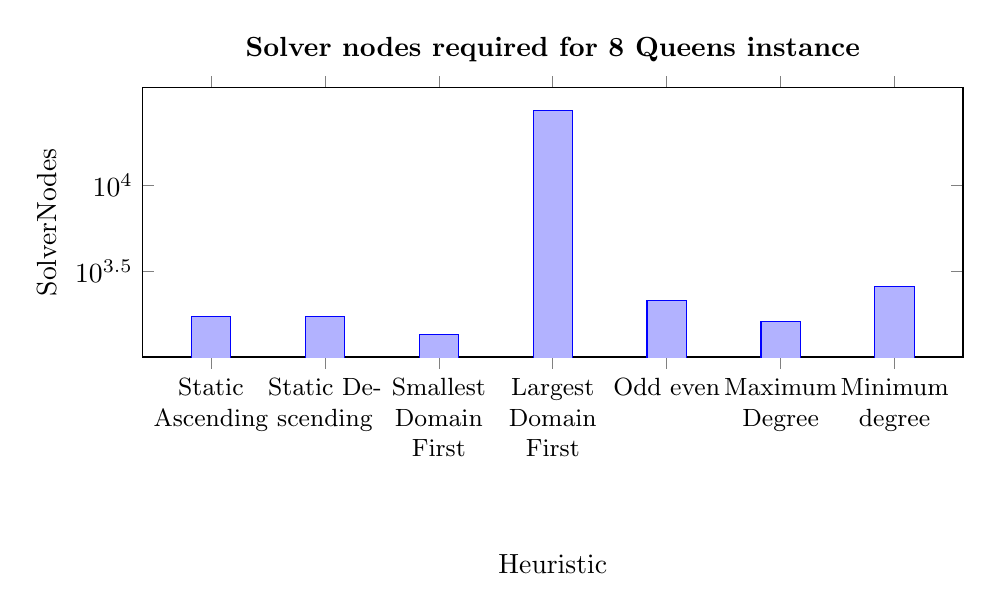
\begin{tikzpicture}
\begin{axis}[
	title = {\textbf{Solver nodes required for 8 Queens instance}},
	bar width=0.5cm,
	ybar,
	legend pos=south east,
	%enlarge x limits=0.4,
	ymode=log,
	ytick={1000,3162,10000},
	height=5cm,
	width=12cm,
	xlabel={Heuristic},
	%xtick={23,24},
	%xticklabels={langfords2-3, langfords2-4},
	xtick=data,
	symbolic x coords = {Static Ascending,Static Descending,Smallest Domain First,Largest Domain First,Odd even,Maximum Degree,Minimum degree},
	x tick label style={font=\small,text width=1.5cm,align=center},
	legend pos=outer north east,
	ylabel={SolverNodes},
	xlabel style={yshift=-1cm}
]

\addplot coordinates {(Static Ascending, 1724) (Static Descending, 1724) (Smallest Domain First, 1360) (Largest Domain First, 27138) (Odd even, 2132) (Maximum Degree, 1612) (Minimum degree, 2592)};

\end{axis}
\end{tikzpicture}
\hspace{1cm}
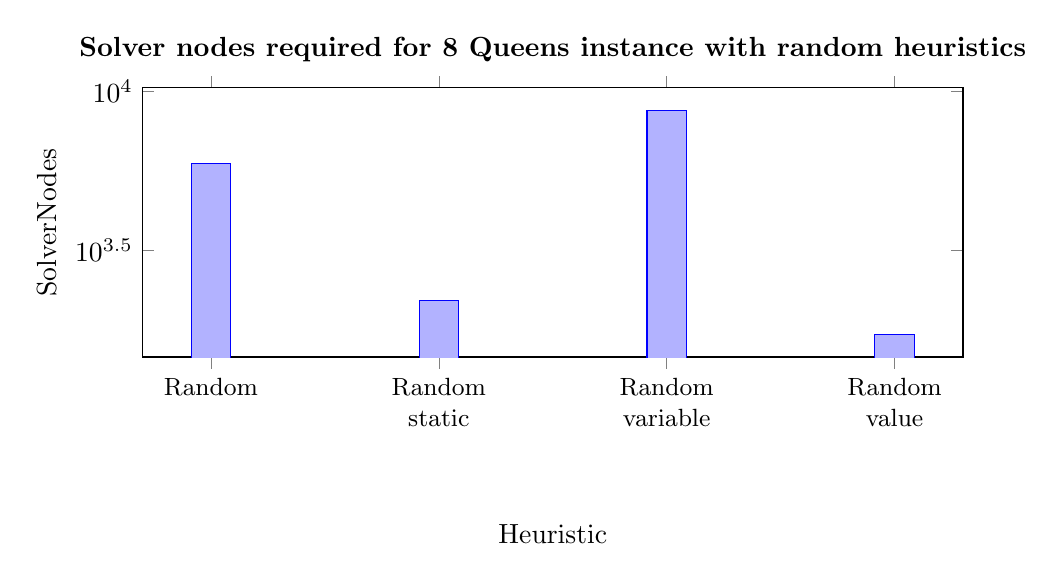
\begin{tikzpicture}
\begin{axis}[
	title = {\textbf{Solver nodes required for 8 Queens instance with random heuristics}},
	bar width=0.5cm,
	ybar,
	legend pos=south east,
	ymode=log,
	height=5cm,
	width=12cm,
	xlabel={Heuristic},
	xtick=data,
	symbolic x coords = {Random, Random static, Random variable, Random value, Smallest Domain First, Largest Domain First},
	x tick label style={font=\small,text width=1.5cm,align=center},
	legend pos=outer north east,
	ylabel={SolverNodes},
	xlabel style={yshift=-1cm}
]

\addplot coordinates {(Random,5942) (Random static,2212) (Random variable,8716) (Random value,1724)};

\end{axis}
\end{tikzpicture}
\caption{Bar plot}
\end{figure}





\begin{figure}[H]
\centering
\sixplot{N queens}{queens2.csv}{\cspplot}
\caption{N queens problem performance with different metrics and heuristics.}
\end{figure}

\begin{figure}[H]
\centering
\sixplot{N queens}{queens.csv}{\randomplot}
\caption{N queens problem performance of random heuristics}
\end{figure}



\subsection{Langfords}
\begin{figure}[H]
\centering
\bargraph{Langfords}{Instance}{SolverNodes}{langfords.csv}
\caption{Langfords problem with different metrics and heuristics.}
\end{figure}

\begin{figure}[H]
\centering
\bargraphrandom{Langfords}{Instance}{SolverNodes}{langfords.csv}
\caption{Langfords problem with random heuristics.}
\end{figure}



\section{Conclusion and evaluation}

\printbibliography

\end{document}



